\documentclass{beamer}

\usetheme{Frankfurt}
\usecolortheme{seagull}

\usepackage{dot2texi}
\usepackage{tikz}
\usetikzlibrary{shapes,arrows}
\usepackage{bookmark}
\usepackage{graphicx}
\usepackage{todonotes}

\def\email#1{{\tt#1}}

\mode<handout>{%
  \usepackage{pgfpages}
  \pgfpagesuselayout{resize to}[a4paper]
}

\title{Applicability of SSM and UML for Designing a Search Application for the British Broadcasting Corporation (BBC)}
\author{Ross Fenning\inst{1}
  \and Huseyin Dogan\inst{2}
  \and Keith Phalp\inst{2}}
\institute{BBC, UK \\ \email{Ross.Fenning@bbc.co.uk}
  \and Bournemouth University, UK \\ \email{\{hdogan,kphalp\}@bournemouth.ac.uk}}
\date{2014-06-17}

\begin{document}

\begin{frame}[plain]
  \titlepage
\end{frame}

% Background
\begin{frame}
  \frametitle{About Me}
  \begin{itemize}
    \pause \item Senior Software Engineer
    \pause \item BBC Future Media
    \pause \item Content Discovery: Search
    \pause \item BBC Academy and University of Bradford, UK
    \pause \item Bournemouth University and Lancaster University
    \pause \item School of Design Engineering \& Computing at Bournemouth University
  \end{itemize}
\end{frame}

\begin{frame}
  \frametitle{What is BBC Search?}
  \framesubtitle{i.e. What do I work on?}
  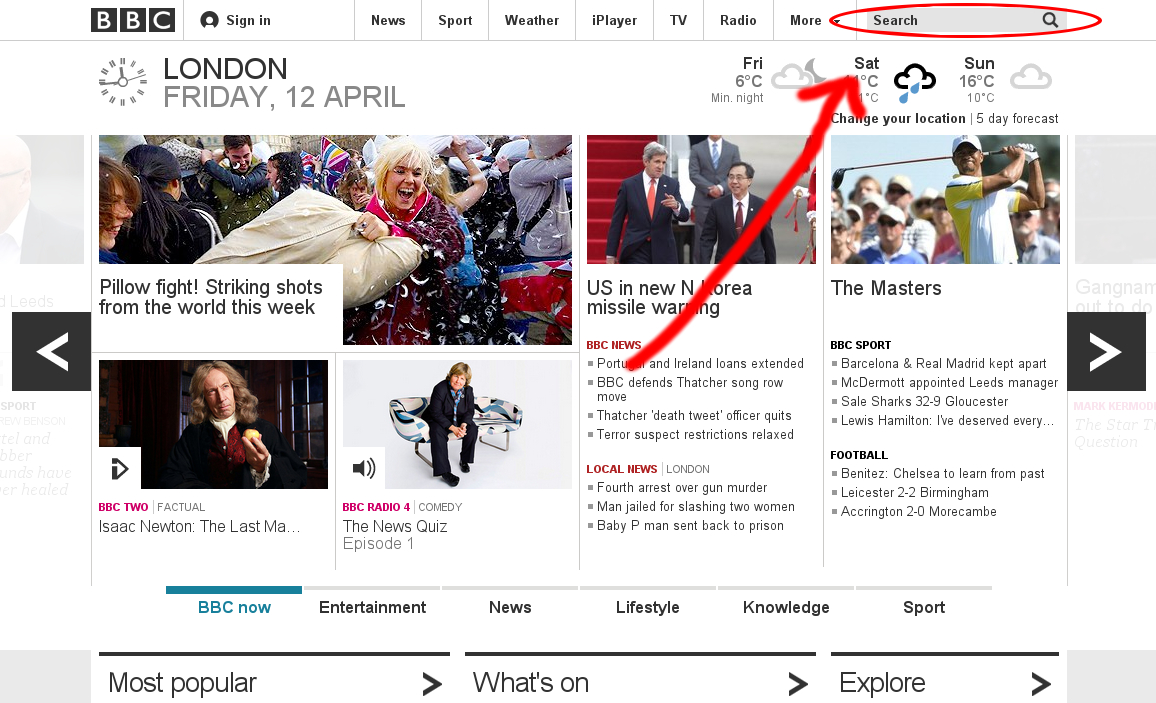
\includegraphics[width=\linewidth]{homepage.png}
\end{frame}

\begin{frame}
  \frametitle{BBC Search results}
  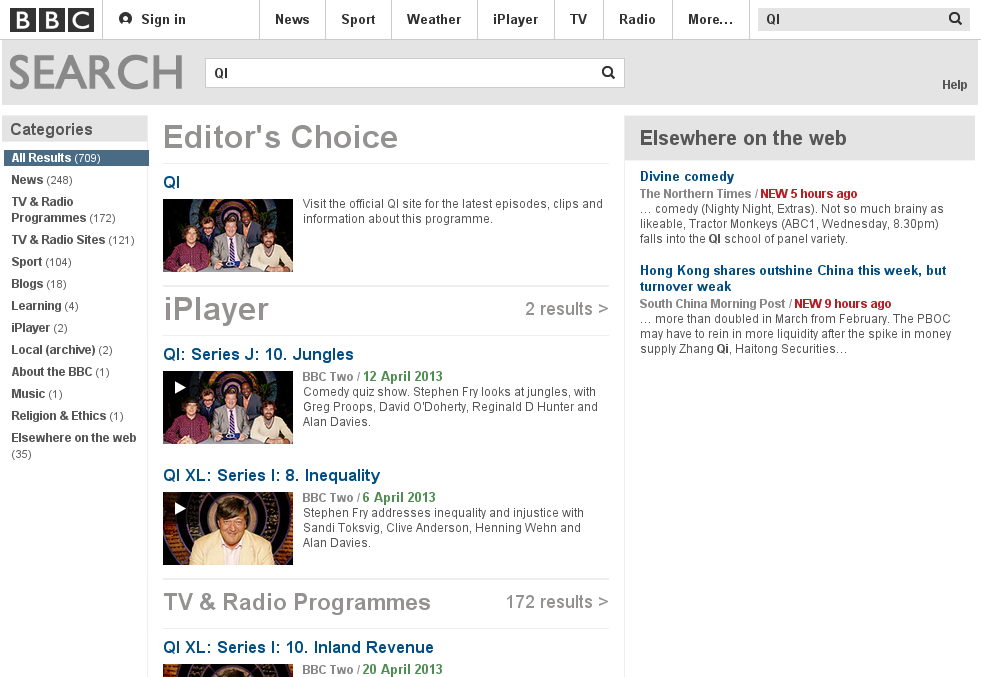
\includegraphics[width=\linewidth]{results.png}
\end{frame}

\begin{frame}
  \frametitle{BBC iPlayer Search results}
  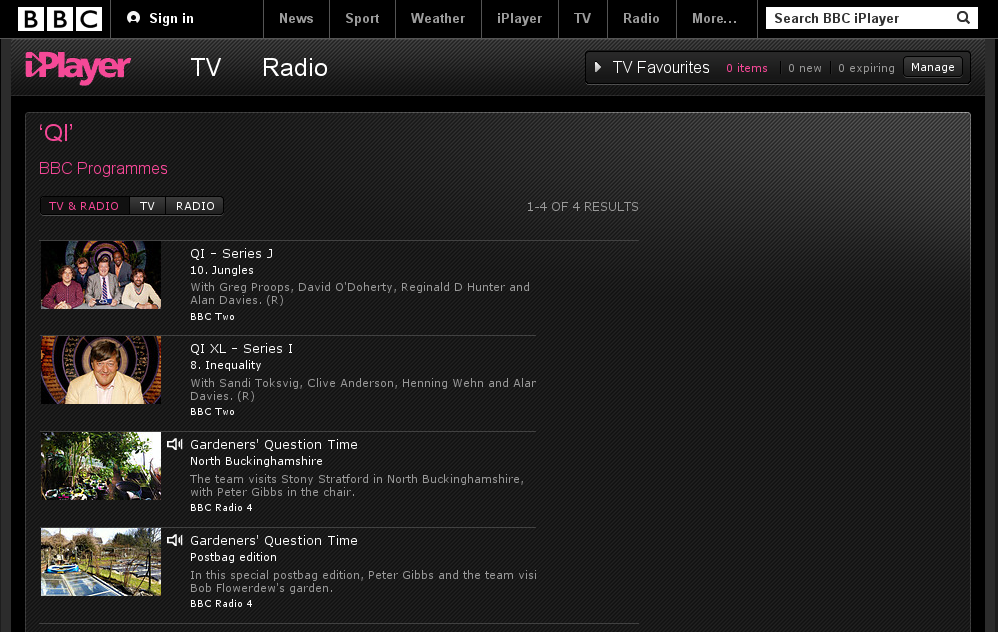
\includegraphics[width=\linewidth]{iplayer.png}
\end{frame}

\begin{frame}
  \frametitle{CBBC Search results}
  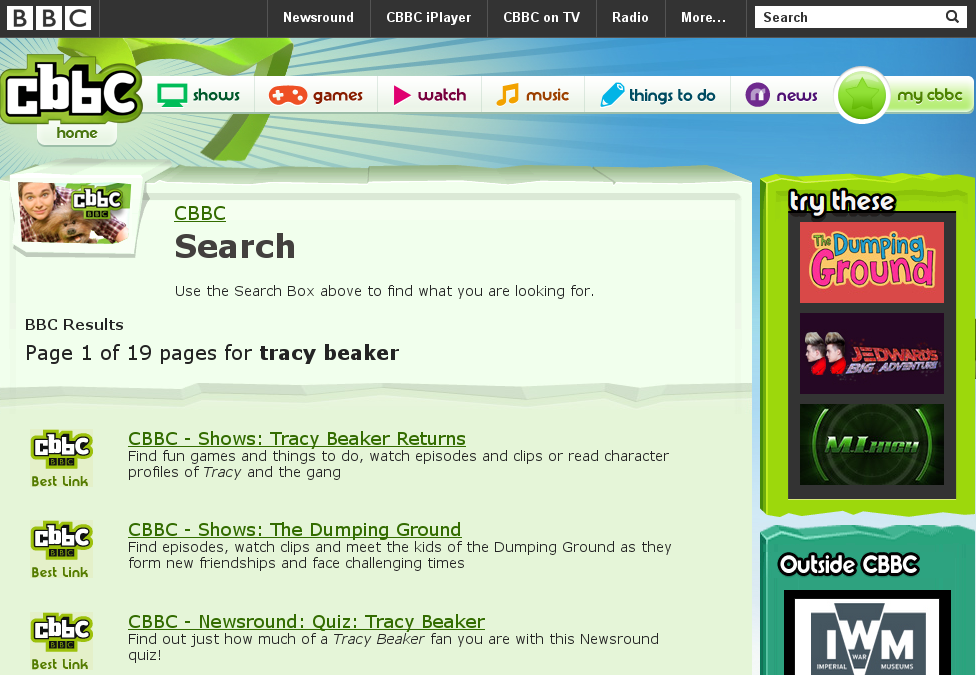
\includegraphics[width=\linewidth]{cbbc.png}
\end{frame}

\begin{frame}
  \frametitle{Why BBC Search?}
  \framesubtitle{Isn't Google good enough?}
  \begin{itemize}
    \pause \item We can search the BBC via Google
    \pause \item What can the BBC offer that Google cannot?
    \pause \item Domain knowledge about our own content
    \pause \item More ``real time'' updates of content
  \end{itemize}
\end{frame}

% Design Goals
\begin{frame}
  \frametitle{Design Goals}
  \framesubtitle{Motivation}
  \begin{itemize}
    \pause \item Showcase possible modelling via high-level thinking and design of a new search application
    \pause \item Take a ``fresh'' approach as if we are replacing the whole system
    \pause \item A new design can (hopefully) inform iterative improvements on a current system
    \pause \item Can SSM give us contextualisation so any modelling and design reflect the real world more appropriately?
    \pause \item Can SSM help us consider the holistic search system that emerges after this integration?
    \pause \item Can SSM ensure that the emergement properties of the whole meet the needs of the UK audience and people within the BBC?
  \end{itemize}
\end{frame}

\begin{frame}
  \frametitle{Design Goals}
  \framesubtitle{Requirements}
  \begin{itemize}
    \pause \item Existing search application serves a wide variety of use cases
    \pause \item The Search application should integrate where possible with other existing systems
    \pause \item Website is very high traffic
    \pause \item Different parts of the overall website are maintained by distinct teams
    \pause \item Varying applications, data stores and content management systems
  \end{itemize}
\end{frame}

\begin{frame}
  \frametitle{Problem Contextualisation through SSM}
  \begin{itemize}
    \pause \item Claim: ``Hard systems'' (e.g. UML) take an ontological view:
    \begin{itemize}
      \pause \item What components are there?
      \pause \item Who are the actors?
      \pause \item What are the interactions between actors and components?
      \pause \item What are the computations or workflows steps/stages?
    \end{itemize}
    \pause \item Claim: SSM takes an epistemological view:
    \begin{itemize}
      \pause \item How does the holistic search system transform user needs to content and information?
      \pause \item How can the purposeful activity be monitored?
      \pause \item How is the activity observed by different observers?
      \pause \item How can different observers inform the activity?
    \end{itemize}
    \pause \item Dogan and Henshaw (2010) showed a transtion from soft systems to hard models
  \end{itemize}
\end{frame}

\begin{frame} 
  \frametitle{Problem Contextualisation through SSM}
  \framesubtitle{Rich Picture}
  \pause 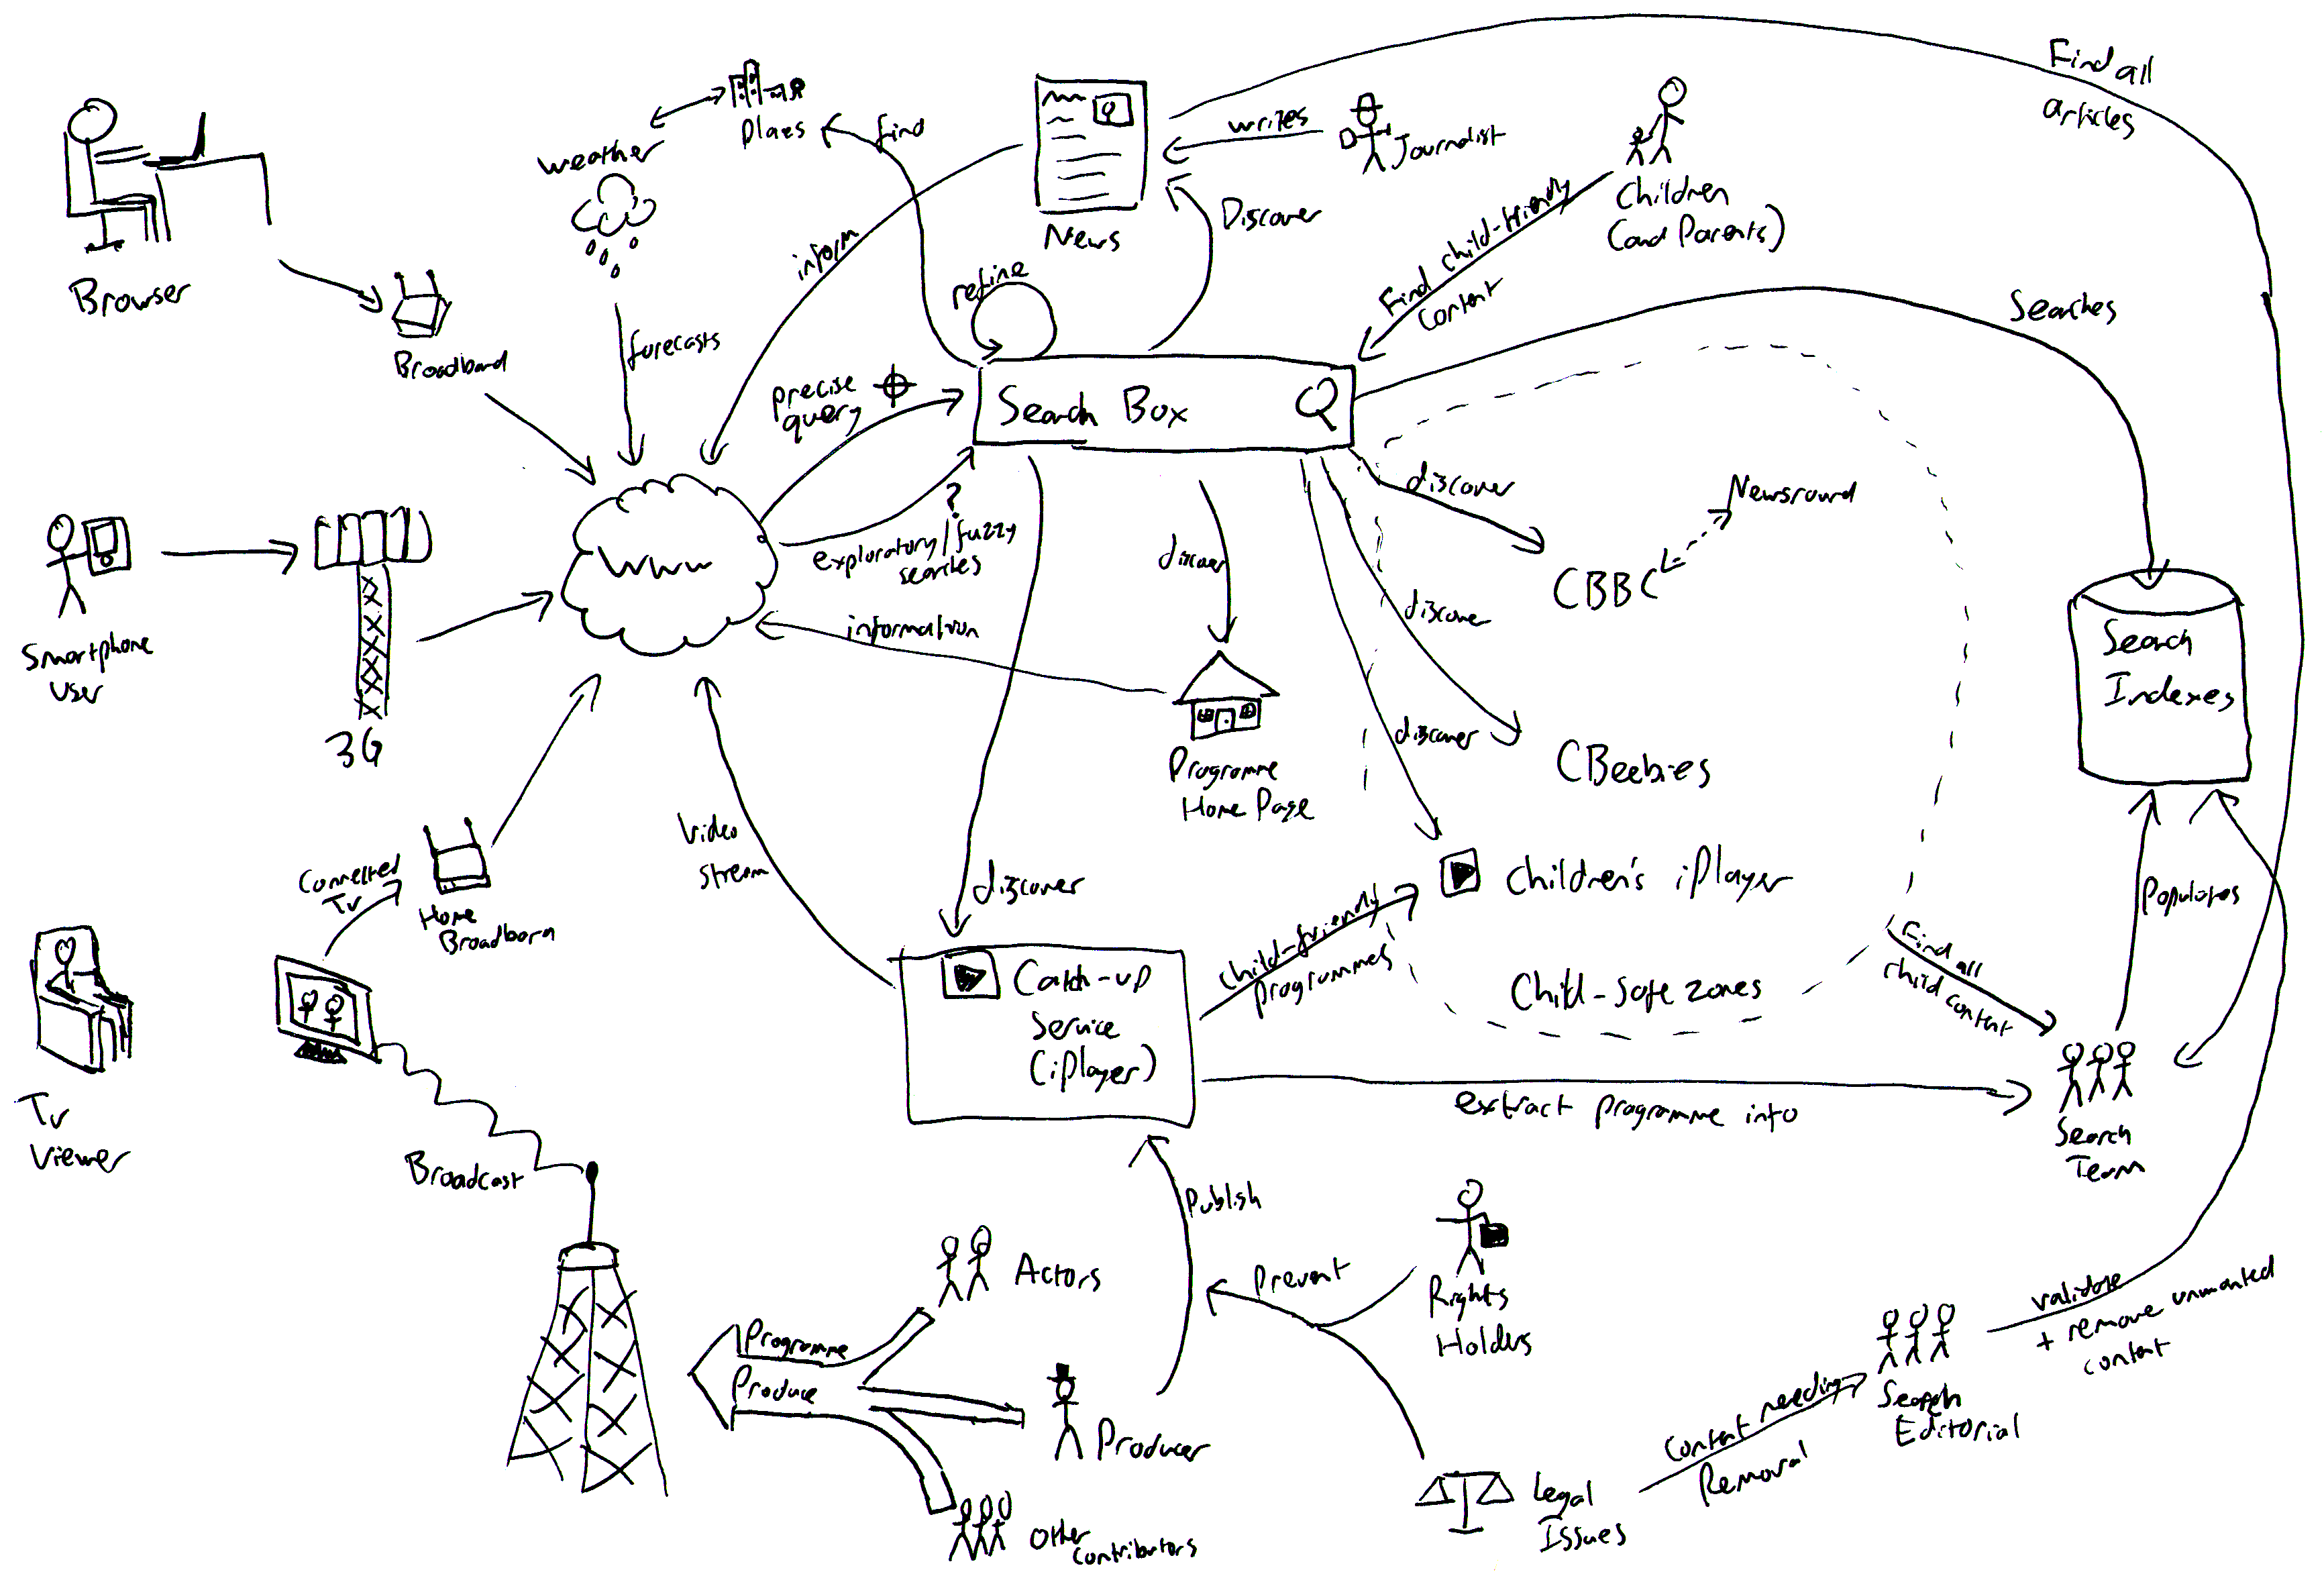
\includegraphics[width=\linewidth]{rich-picture.png}
\end{frame}

% Extracting use cases
\begin{frame}[fragile]
  \frametitle{Use Case Extraction}
  \framesubtitle{Identifying users}
  \begin{center}
    \begin{dot2tex}[dot,scale=0.6]
      digraph G {
        rankdir=LR;
        node;
        "Rich Picture" -> Users
        Users -> "Direct Users";
        Users -> "Indirect Users";
      }
      \end{dot2tex}
    \quad
  \begin{itemize}
    \pause \item Identify all users of the system in the rich picture
    \pause \item Separate \emph{direct} users from \emph{meta-level} users
    \pause \item Direct use cases should emerge from the rich picture
    \pause \item NOTE: This separation is still \emph{subjective} and use cases may change as the rich picture changes
  \end{itemize}
    \end{center}
\end{frame}

% Designing behaviour for indirect users
\begin{frame}
  \frametitle{Use Case Extraction}
  \framesubtitle{Meta-level Users}
  \begin{itemize}
    \pause \item Meta-level users do not transition to the use case models directly
    \pause \item We should still consider how meta-level users are affected by emergent properties of the holistic system
  \end{itemize}
\end{frame}

% Designing behaviour for direct users
\begin{frame}
  \frametitle{Use Case Extraction}
  \framesubtitle{Direct Users}
  \begin{itemize}
    \pause \item Direct users transition directly to actors into a UML use case diagram
    \pause \item Use cases should derive from and be justifiable by the rich picture
    \pause \item Direct users divide up into \emph{content production} and \emph{audience}
    \pause \item Examples of each:
    \begin{itemize}
      \pause \item Producers of TV programmes metadata
      \pause \item Users of the search web application
    \end{itemize}
  \end{itemize}
\end{frame}

\begin{frame}
  \frametitle{Use Case Extraction}
  \framesubtitle{UML Use Case Diagram}
  \pause \includegraphics[width=\linewidth]{use_case.png}
\end{frame}

\begin{frame}
  \frametitle{System Behaviour}
  \framesubtitle{Programmes metadata producer}
  \pause \includegraphics[width=\linewidth]{plant_sequence_producer.png}
\end{frame}

\begin{frame}
  \frametitle{System Behaviour}
  \framesubtitle{Website user}
  \begin{center}
    \pause \includegraphics[height=0.8\textheight]{plant_sequence_user.png}
  \end{center}
\end{frame}

\begin{frame}
  \frametitle{System Behaviour}
  \framesubtitle{Lazy-loading page via AJAX}
  \begin{center}
    \pause \includegraphics[height=0.8\textheight]{plant_sequence_ajax.png}
  \end{center}
\end{frame}

% Domain modelling for search -- model business rules as per benefits shown in background, but also keep it generic
\begin{frame}
  \frametitle{Domain Modelling}
  \begin{itemize}
    \pause \item Use cases identify types of content users want to search
    \pause \item Ontology designs exist for specific content domains, e.g. programmes, sport
    \pause \item A search across all content types needs a model to span all domains
  \end{itemize}
\end{frame}

\begin{frame}
  \frametitle{Domain Modelling}
  \framesubtitle{Class Diagram}
  \begin{center}
    \pause \includegraphics[height=0.8\textheight]{plant_model.png}
  \end{center}
\end{frame}

% Discussion and Analysis -- Use cases - More SSM needed?

\begin{frame}
  \frametitle{Discussion}
  \framesubtitle{Use Cases}
  \begin{itemize}
    \pause \item Use case model seems justifiable at a high level
    \pause \item Many use cases and variations are missing
    \pause \item More collaborative and continuous use of SSM should incorporate respective domain experts
    \pause \item More user testing, audience feedback, requirements-gathering, etc. needed
    \pause \item Possible need to iterate SSM processes towards a collection of use case models
  \end{itemize}
\end{frame}

\begin{frame}
  \frametitle{Discussion}
  \framesubtitle{System Behaviour}
  \begin{itemize}
    \pause \item Enterprise Integration patterns
    \begin{itemize}
      \pause \item Asynchronous messaging
      \pause \item Claim Check -- Store absolute minimum information to function and maintain references to source systems
      \pause \item Content Enricher -- Replicate information from other systems redundantly
      \pause \item Index vs. warehouse?
      \pause \item How to evaluate the better approach?
    \end{itemize}
  \end{itemize}
\end{frame}

% Discussion and Analysis -- Domain Model -- Polymorphism
\begin{frame}
  \frametitle{Discussion}
  \framesubtitle{Domain Model}
  \begin{itemize}
    \pause \item Large, fully-inclusive data model useful mainly as communication artefact
    \pause \item Aggregate models hard to keep in sync with changes in respective domains
    \pause \item We can extract a polymorphic supertype containing only properties needed for a search application
    \pause \item We can go further and model a ``Search Result'' facade
  \end{itemize}
\end{frame}

% Discussion and Analysis -- Domain Model -- Duck Typing
\begin{frame}
  \frametitle{Discussion}
  \framesubtitle{Schemalessness and Duck Typing}
  \begin{itemize}
    \pause \item Statically typed approach: A \emph{Place} always has a ``today's weather forecast'' attribute
    \pause \item Dynamically (``duck'') typed approach: any entity can have a ``today's weather forecast'' attribute and we display this forecast if that attribute is present
    \pause \item Allows other entities in future to have forecasts too (e.g. \emph{Events} such as football matches)
    \pause \item Search application can store all fields from upstream sources and choose when to start using them
  \end{itemize}
\end{frame}

% Discussion -- More SSM: 3 Es?
\begin{frame}
  \frametitle{Discussion}
  \framesubtitle{Overall Model}
  \begin{itemize}
    \pause \item Promising at a high level
    \pause \item Agile methodology would encourage developing prototype or MVP to test assumptions early
    \pause \item Lacking suitable ``monitoring'' of the system as taught by SSM, e.g. Checkland's ``3 Es'' (efficacy, efficiency, effectiveness)
  \end{itemize}
\end{frame}

% Shortcomings -- Performance? NFRs?
\begin{frame}
  \frametitle{Evaluation and Difficulties}
  \framesubtitle{Non-functional Requirements}
  \begin{itemize}
    \pause \item BBC is a high-traffic website
    \pause \item Content such as news articles are published frequently
    \pause \item How to model requirements around performance, robustness and latency?
  \end{itemize}
\end{frame}

% Shortcomings -- Agile?
\begin{frame}
  \frametitle{Evaluation and Difficulties}
  \framesubtitle{Detailed Design and Agile}
  \begin{itemize}
    \pause \item Models developed at such a high level lack detailed design (not surprisingly)
    \pause \item Agile methodologies encourage designing and delivering a small part of the system early
    \pause \item Detailed design emerges in response to feedback and change
    \pause \item Hard models can be altered in time with these iterations
    \pause \item We can defer outstanding questions about hard models until we might have more information
    \pause \item This seems in line with the continuous feedback cycles within SSM
  \end{itemize}
\end{frame}

% Validation?

% Further Work
\begin{frame}
  \frametitle{Further Work}
  \begin{itemize}
    \pause \item How can the models be effectively validated?
    \pause \item Can the rich picture and use of SSM be repeated and expanded with input from a wider range of experts?
    \pause \item How will the models change when this happens?
    \pause \item Are there more parallels between Agile and SSM that engineers in industry have yet to appreciate?
    \pause \item Should more development processes be considered alongside SSM and UML? e.g. RUP (OpenUP) or AUP?
  \end{itemize}
\end{frame}

\end{document}
